\documentclass[tikz,border=8pt]{standalone}
\usetikzlibrary{arrows.meta,calc,positioning,patterns}
\begin{document}
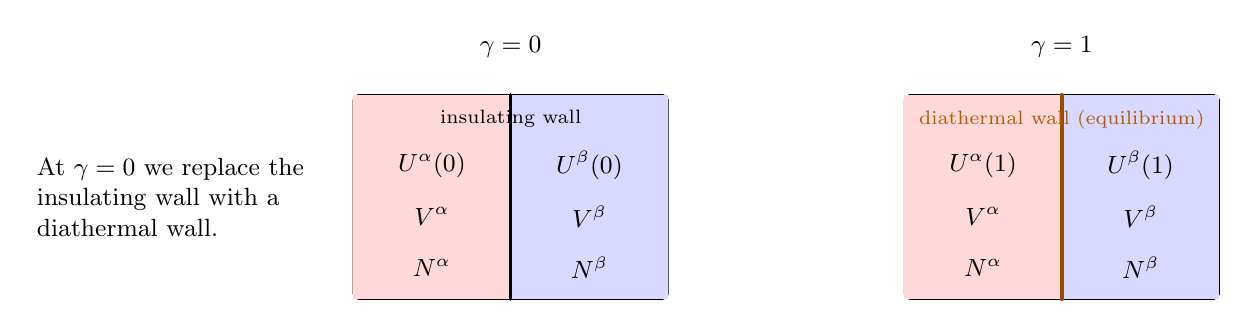
\begin{tikzpicture}[font=\small,line cap=round]
  % Left configuration gamma=0
  \node at (-3.5,2.4) {$\gamma=0$};
  \draw[rounded corners=2pt,fill=gray!5] (-5.5,-0.8) rectangle (-1.5,1.8);
  \path (-3.5,-0.8) -- (-3.5,1.8) coordinate (mid0);
  \fill[red!15] (-5.5,-0.8) rectangle (-3.5,1.8);
  \fill[blue!15] (-3.5,-0.8) rectangle (-1.5,1.8);
  \draw[very thick] (-3.5,-0.8) -- (-3.5,1.8);
  \node at (-4.5,0.9) {$U^\alpha(0)$};
  \node at (-4.5,0.25) {$V^\alpha$};
  \node at (-4.5,-0.4) {$N^\alpha$};
  \node at (-2.5,0.9) {$U^\beta(0)$};
  \node at (-2.5,0.25) {$V^\beta$};
  \node at (-2.5,-0.4) {$N^\beta$};
  \node[below=2pt of mid0] {\scriptsize insulating wall};
  \node[left=6pt of mid0] {};
  \node[align=left,anchor=east] at (-6,0.5) {At $\gamma=0$ we replace the\\ insulating wall with a\\ diathermal wall.};

  % Right configuration gamma=1
  \node at (3.5,2.4) {$\gamma=1$};
  \draw[rounded corners=2pt,fill=gray!5] (1.5,-0.8) rectangle (5.5,1.8);
  \path (3.5,-0.8) -- (3.5,1.8) coordinate (mid1);
  \fill[red!15] (1.5,-0.8) rectangle (3.5,1.8);
  \fill[blue!15] (3.5,-0.8) rectangle (5.5,1.8);
  \draw[very thick,orange!60!black] (3.5,-0.8) -- (3.5,1.8);
  \node at (2.5,0.9) {$U^\alpha(1)$};
  \node at (2.5,0.25) {$V^\alpha$};
  \node at (2.5,-0.4) {$N^\alpha$};
  \node at (4.5,0.9) {$U^\beta(1)$};
  \node at (4.5,0.25) {$V^\beta$};
  \node at (4.5,-0.4) {$N^\beta$};
  \node[below=2pt of mid1,orange!70!black] {\scriptsize diathermal wall (equilibrium)};
\end{tikzpicture}
\end{document}
